\section{Module 12. Oblique imaging}

\indent The literature to this module is as useful as nipples on
men. Everything is about inventing how to realize point 1. of the
list. \\
 \indent Oblique Imaging is a technique to create non-perspective
projections from 3D or multiple 2D images.\\

\indent In order to create oblique image it is essential to: 
\begin{itemize}
\item choose two angles under which the plane will be inclined, 
\item create a matrix of points that this plane consists of, 
\item from existing points pick those, which will be used in the image, 
\item interpolate points that are not existing. 
\end{itemize}
\indent Type of interpolation can vary, but in this project interpolation
based on mean will be used. To interpolate one pixel mean of all pixels
around him with given proximity is taken.

\begin{figure}[H]
\centering{}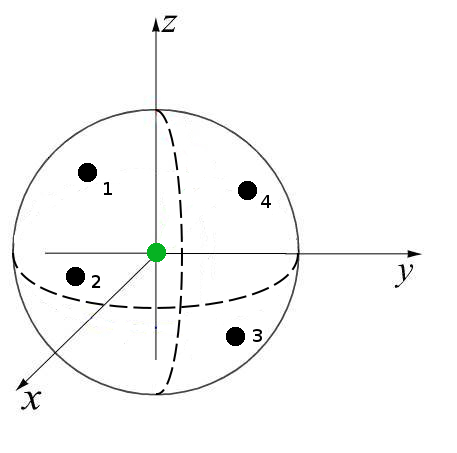
\includegraphics[scale=0.7]{figures/m11_spherexyz}\caption{Visualization of pixels taken to interpolate}
\label{fig:figures/m11_spherexyz } 
\end{figure}